\chapter{Runtime Verification}
\label{chap:Runtime Verification}

In this chapter, we introduce a software validation technique known as runtime verification and explain how it is used to detect software defects.  We examine the unique characteristics that make it valuable among other validation techniques and the associated computational cost.  Then we consider the needs of an Android security system and how we can adapt runtime verification to detecting security breaches instead of software defects.

\section{The Problem of Defects}

Runtime verification is one of many responses to the problem of defects.  A defect is an unwanted system behaviour that falls outside the specification.  Due to their ubiquity, software defects are overlooked by society when they result in nothing more serious than delays and frustrations.  We accept a failure as mere inconvenience when the result is a delayed train, an out-of-order cash machine, or the need to repeat an entry into a website.  But, the problem of defects becomes more serious when system failures are costly, deadly, or invasive, and automatic control systems find their way into virtually every aspect of our daily lives.

By the late 1960s, the cost of developing software had become greater than the cost to develop hardware.  The phenomenon was named `the software crisis'.  Nowadays, people speak about `the software quality crisis' being where the cost of verifying the correctness of software is greater than the cost of writing software.  In the field of software quality assurance, cost-effective validation techniques are in high demand.

Measuring the defect rate is essential if we are to find effective solutions.  The cause of a defect may be rooted in any of the development stages, but once development has reached the implementation stage, it becomes possible to use the KLOC metric.  KLOC measures the number of defects a developer introduces per thousand lines of delivered code.  When Steve McConnell studied this topic for his book, Code Complete, he arrived at an average defect rate across the software development industry of between 1 and 25 defects per 1000 lines of delivered code \cite{CodeCompleteKLOC}.  The author of this paper can say from 20 years of personal experience in the software development industry that Code Complete is a widely read, well-regarded book, and the figure measured by McConnell is broadly accepted.  More recent measures of faults per line of code show the problem has not improved \cite{BattleOfTheBugs} \cite{Coralogix} \cite{sogetilabs}.


\section{Countermeasures}

It is no surprise that defects plague software development, but with a measure of defect rate, we can grade the efficacy of different approaches to solving the defect problem.  Some of those approaches are:

\begin{enumerate}
\item Software testing.
\item Peer review in the form of code walk-throughs and inspections.
\item The application of measurable coding standards to reduce complexity metrics such as McCabes cyclomatic complexity \cite{CodeCompleteMcCabe}.
\end{enumerate}

\noindent None of these methods can guarantee that all faults will be discovered relative to a given specification.\\

\subsection{Software Testing}
\label{subSec:Testing}

The most common validation method is testing.  Being a dynamic analysis technique, testing is performed on a system while it is running.  Tests can be generated automatically from a specification but are more commonly generated manually during the development cycle.  To ensure their integrity, independent quality assurance teams must generate and administer tests rather than the software developers.  There are several subcategories: black box, white box, and unit testing; each has its own characteristics.  When black box testing, the QA team has no visibility of the source code; they only use the specification to direct the tests they run.  In the case of white box testing, the QA team can inspect the source code before deciding upon which tests to perform.  Unit testing automates the execution of tests by the test itself being a program that accepts a fragment of the source code as a parameter, otherwise, execution of tests is also manual.  When tests are administered manually the code under test does not require modification but, when executing tests automatically by unit testing, additional development effort is required to produce unit tests.  It may also be necessary to produce mock implementations of subroutines that are required during the test but are not the subject of the test.  And the design of the code under test can also be impacted because it must be possible to substitute subroutines for mocks.  Producing unit tests requires significant development expertise.  The integrity of unit testing is compromised if developers also develop the tests because the QA team lacks the expertise.

But the Achilles heel of testing is common to all categories.  That is, for testing to be complete, a test is required for every possible input to the system.  This means a test for each functional requirement and every possible failure mode.  Regardless of whether testing is manual or automated, testers often assume a testing hypothesis as follows: Provided a system passes finite test cases, then the system is correct for all inputs.  This hypothesis is often not proven but just casually assumed.  Generally, the number of failure modes is too large to cover, or infinite, and therefore it is impossible to test all inputs to the system.  Thus safety and security cannot be guaranteed.  When white box testing, the QA team can use knowledge of the code to judge which inputs it is sensitive to and filter out the rest.  But this can only lessen the coverage problem.

\subsection{Peer Reviews}
\label{subSec:PeerReviews}

Peer reviews are essentially an informal version of static code analysis, they are shown to improve code quality \cite{CodeCompleteCodeReviews} but, the scope and intensity of the analysis are left to the reviewer and so cannot be guaranteed to be complete.\\

%\subsection{Measurable Coding Standards}
%\label{subSec:MeasurableCodingStandards}

\noindent Next, there are formal static analysis methods like code validation using software model checking or code proving tools.  These techniques have their own advantages and limitations:

\subsection{Model Checking}
\label{subSec:ModelChecking}

Software model checking extracts an abstract model of a piece of software from the source code.  The model covers every possible state following the execution of each instruction.  Correctness properties are formulated manually to express a specification, then automated model proving techniques ensure that all possible executions of the code satisfy those properties.  Model checking has a valuable advantage in that the complete behaviour, including all requirements and failure modes, of a system can be examined because the model covers all inputs to the system.  Developers can perform model checking without compromising the integrity of the result because construction and analysis of the model are automated by trusted processes.  NASA successfully used model checking to verify Java bytecode in the 2005 Java Pathfinder \cite{JavaPathfinder} project.  But they concur that it is infeasible for all but the smallest systems of between 10 and 100 KLOC, the reason being that model checking suffers from the state explosion problem, meaning there are too many possible states to cover, and the task of analysing all possible executions becomes colossal when dealing with larger systems.

\subsection{Program Provers}
\label{subSec:ProgramProvers}

Validation using code provers such as Microsoft Dafny\footnote{\url{https://www.microsoft.com/en-us/research/project/dafny-a-language-and-program-verifier-for-functional-correctness/}}, KeY\footnote{\url{https://www.key-project.org/}}, or Spark ADA\footnote{\url{https://www.adacore.com/about-spark}}, entails the developer manually augments the source code with a formal specification and derives proofs regarding the correct functioning of the software.  The technique operates on the source code, and while third-parties can disassemble and decompile source code, the compilation process often discards symbols and may intentionally obfuscate the code.  The decompilation process will be unable to reconstruct the original code verbatim.  Without a specification and obfuscated code, the problem presented to the third-party developer becomes akin to reverse engineering.  For this reason, it is a technique best suited to use by the original developer during the development stage.

Being a static analysis technique means code provers benefit from validation of all inputs to the system.  But, in practice, the augmentations can exceed the code.  Development effort to reach proof is high and, to limit cost, it is common for only a select few requirements to be proven.\\

\noindent Table \ref{table:VerificationTechniquesSummarised} summaries the comparison of different verification technique with regard to relevant attributes.

\begin{table}[h!]
\resizebox{\columnwidth}{!}{
\begin{tabular}{p{0.18\linewidth} p{0.135\linewidth} p{0.135\linewidth} p{0.135\linewidth} p{0.15\linewidth} p{0.15\linewidth} p{0.21\linewidth}}
\hline
& Black Box Testing & White Box Testing & Unit Testing & Model\hspace{0.2\linewidth} Checking & Program Provers & Runtime\hspace{0.4\linewidth}Verification\\
\hline
Additional Code Required & No & No & Yes & No & Yes & Monitor required  \\
Source Required & No & Yes & Yes & Yes & Yes & Only if logging is not automatic \\
Complete\hspace{0.2\linewidth}Coverage & No & No & No & Yes & Complete for selected requirements & No \\
Degree of\hspace{0.3\linewidth}Requirement Coverage & Each\hspace{0.6\linewidth}requirement\hspace{0.3\linewidth}needs a test &  Each\hspace{0.6\linewidth}requirement\hspace{0.3\linewidth}needs a test  &  Each\hspace{0.6\linewidth}requirement\hspace{0.3\linewidth}needs a test  & All\hspace{0.6\linewidth}requirements covered & Select\hspace{0.6\linewidth}requirements covered & Select\hspace{0.6\linewidth}requirements covered \\
Performed By & Independent QA & QA & QA & Developer & Developer & Independent QA \\
Performed\hspace{0.2\linewidth}During & Development cycle & Development cycle & Development cycle & Development cycle & Development cycle & Runtime \\
Degree of\hspace{0.3\linewidth}Automation & Automated generation from a specification is possible & Automated generation of inputs & Manual test generation.  Automated test execution & Manual property expression.  Automated model generation, and model checking & Manual proof construction.  Automated evaluation. & Manual logging, property expression, and intervention.  Automated monitor generation, and property evaluation\\ \hline
\end{tabular}
}
\caption{Attributes of Verification Techniques Summarised}
\label{table:VerificationTechniquesSummarised}
\end{table}

\section{Runtime Verification as an Alternative}

% traces are finite in size - an infinite number of finite prefixes of an infinite trace rather than a finite (single) infinite trace.  Consider a finite trace as an incrementally observed finite prefix of an unknown infinite trace.
% considers only a subset of total possible executions - similar in that regard to testing
% avoids state explosion problem of model checking but can suffer if monitors are Buchi automata based FSM.
% offline or realtime monitoring possible.

Runtime verification occupies a unique position among verification techniques, shown in figure \ref{fig:VerificationTechniqueTree} below.  It is a dynamic analysis technique, in other words, it operates on software while it is running instead of on the source code.  A software entity called a monitor is generated that acts as a watchdog for the system to be verified.  The monitor will raise an alert if a correctness property $\varphi$ is violated.  Correctness properties are formulated to express the safe or secure running of the system.  A property will either specify a correct execution that must be maintained or specify a failure mode that should be prevented.  For example, if the system to be verified is a motorcar, then the seatbelts must be engaged when the vehicle is in motion.  A correctness property would express this rule.  The monitor observes the system and evaluates whether the observed execution satisfies the property.  If not, the monitor can raise an alert or intervene.

\begin{figure}[h!]
	\resizebox{\columnwidth}{!}{%
	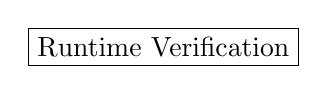
\begin{tikzpicture}
	\tikzset{level distance=75pt}
	\Tree [.{Verification}
	        [.{Static Analysis}
	            [.{Informal}
	            	[.{Peer Review} ]
				]
	            [.{Formal}
	            	[.{Model Checking} ]
	            	[.{Program Provers} ]
	            	[.{Code Metrics} ]
				]
	        ] 
			[.{Dynamic Analysis}
				[.{Code Required}
					[.{Manual Execution}
						[.{White Box Testing} ]
					]
					[.{Automatic Execution}
						[.{Unit Testing} ]
					]
				]
				[.{Code Not Required}
					[.{Manual Execution}
						[.{Black Box Testing} ]
					]
					[.{Automatic Execution}
						[.\node[draw]{Runtime Verification}; ]
					]
				]
			]
		]
	\end{tikzpicture}%
	}
	\caption{Runtime Verification Among Other Verification Methods}
	\label{fig:VerificationTechniqueTree}
\end{figure}

Observation of the system requires visibility of the state of the system or the events leading to state changes.  To achieve this, it must be possible to create a log of events.  For brevity, we will describe log entries as events.  The monitor then evaluates whether the trace satisfies the property.  Offline monitoring evaluates a trace after execution has finished and the trace has been captured.  Realtime monitoring evaluates a property over a trace during execution.

%We will use Linear Temporal Logic \cite{Pnueli} to express properties therefore we must use a variety of LTL that operates on finite traces.  We go into detail on LTL in chapter \ref{chap:Linear Temporal Logic}.

When the monitor evaluates a property over a trace, the trace is always finite in length.  When monitoring offline, we are not concerned because execution finished before evaluation, so no more events will ever occur.  Thus the captured finite trace is complete.  But realtime monitoring can continue indefinitely, and therefore the trace can grow to infinite length.   This disparity must get resolved.  With regard to realtime monitoring, traces are considered to be finite but of continuously increasing length.  After each new event, there is a new trace from the concatenation of the previous trace and the new event.  Thus, when monitoring in realtime, there are infinitely many finite traces, where each is the prefix of a single infinite trace.

In either case, the monitor operates only on observed executions rather an operating on all possible executions.  The state explosion problem that model checking suffers from is avoided but, like other dynamic analysis techniques, runtime verification is incomplete.

A valuable feature of runtime verification is that it can be mostly automated because correctness properties do not have to be formulated by the original developer and, monitors are typically \textit{generated} from correctness properties.  The generation process is assumed to be correct, therefore it will produce a correct monitor.  While the applications to be monitored are assumed to be less reliable because we can say nothing about their construction other than it is recognised that all software contains mistakes, and therefore we assume they are not correct.

Another valuable feature is that this can all be achieved without access to the source code so long as the system logs its activity.  Thus, runtime verification enables existing software to be verified by entirely independent parties.\\

\noindent Runtime verification offers a lightweight approach to verification that is akin to black box testing but the automation aspect makes it more cost-effective.

\subsection{Monitor Construction}

Properties to be monitored are often expressed as finite state machines, regular expressions or linear temporal logic formulae.  For a given property, monitors can be constructed as finite state machines from \Buchi\ automata.  Figure \ref{fig:FSMConstruction} below shows the steps involved when constructing a monitor in this way.

\begin{figure}[h!]
  \centering
  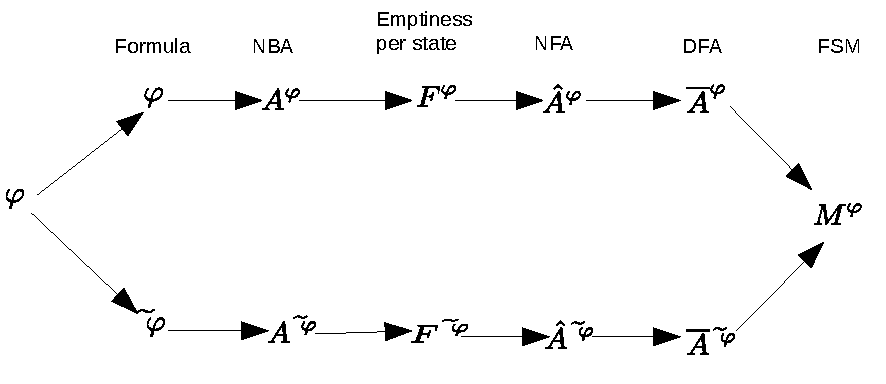
\includegraphics[width=\textwidth]{graphics/BuchiContructionFlow}
  \caption{FSM Based Monitor Construction For a Given Property $\varphi$\cite{RVForLTLAndTLTL}}
  \label{fig:FSMConstruction}
\end{figure}

Two non-deterministic \Buchi\ automata (NBA) are generated from a property supplied as an LTL formula.  One NBA is constructed from the property and the second from its complement.  Emptiness checking is then performed for each NBA by a function that returns $\top$ if the language of the automaton for a given starting state is non-empty.  Using those functions, non-deterministic finite automata (NFA) are defined followed by equivalent deterministic automata (DFA) for both the property and the complement.  These are combined to yield the final finite state machine.

\subsection{Monitor Complexity}

Complexity is a problem for monitors constructed in this manner.  The second step of construction where NBA get generated is subject to the problem of exponential state blow-up.  The fifth step, which generates deterministic finite automata, also suffers from exponential blow-up.  In the worst case, these two steps lead to the size of the final FSM being $O(2^{2^n})$ \cite{RVForLTLAndTLTL}, thus in the worst case it is too complex.  In practice, however, many monitors generated in this way have lower complexity than the worst case and are useful.  We aim to avoid the exponential blow-up problem entirely by using an alternative technique to generate the monitor.

Regardless of how the monitor is generated, there is always a performance penalty to using runtime verification.  At the very least the system will run slower when it is being monitored because it must log it's activities.  This could be the only performance cost if evaluation of the property happens after execution has finished.  Likewise, it is not essential that the monitor runs on the system being monitored.  But, if monitoring is performed in realtime and on the system being monitored, then the computational cost of running the monitor pushes the performance penalty higher still.  Estimates are that runtime verification can slow a system to half its normal speed.

\section{Application of Runtime Verification to Security}

We categorise a security breach as a failure mode of the system.  The properties we formulate will get satisfied when a security breach occurs and get violated under correct operation.  We aim to recognise security breaches as they happen and ideally before they are complete.  If a property describes the events immediately before a security breach then, the monitor can raise an alert so that preventative measures can stop the imminent security breach from ever occurring.  To achieve this, we must evaluate properties in realtime and on the Android system.  There is great emphasis on a computationally efficient algorithm.

Due to the aforementioned requirement, we will not be generating \Buchi\ automata to evaluate a property.  Instead, we will introduce an algorithm in chapter \ref{chap:Rosu-Havelund Algorithm} that promises to reduce complexity to a practically usable class.  In Chapter \ref{chap:Runtime Verification with the Rosu-Havelund Algorithm} we will investigate the algorithm's complexity.

\subsection{Pegasus}

Pegasus is spyware that was discovered in 2016.  A mainstream media expose\'e \cite{PegasusGuardian} claims Pegasus has infected at least 1400 devices belonging to people in government and journalism.\\

What we know about Pegasus on Android\cite{PegasusOnAndroid}:

\begin{itemize}
\item After the infected device boots, Pegasus looks for configuration settings by parsing query string parameters from a URL in the browser's history or reading a file present on the device.
\item It gathers information by querying the databases of messaging and communication apps.
\item It can actively take images from the camera.
\item It will eavesdrop on the user by answering calls from specific numbers without indicating a call is in progress.
\item It sends information to an attacker via a network connection.
\end{itemize}

In the context of Pegasus, we speculate that our runtime verification approach could successfully detect at least some Pegasus attacks:  We reason that threats require the use of the operating system to access resources because Android runs on a diverse array of hardware, and the O/S is the only unified means to access resources.  Consequently, the Pegasus spyware works at the operating system level.  We will warn the user if any security-sensitive resource gets used without user interaction.
